\chapter{Methodology} % Main chapter title

\label{Chapter4} % Change X to a consecutive number; for referencing this chapter elsewhere, use \ref{ChapterX}

\section{Phenanthrene Parameterization}\label{parame}

The two parameterization strategies for ring molecules described in section \ref{parsaft} were implemented for phenanthrene. For both of them, only vapor pressure data \cite{pvphen} was used due to the unavailability of saturated liquid density. The attractive parameter $\lambda _{a}$ was set to six to avoid correlation with the repulsive parameter. The parameterization with the ring equation of \citeonline{muller2017} was done with the number of segments fixed in 5 since this level of coarse graining was also used for the similar molecule anthracene:
\begin{figure}[th]
\centering
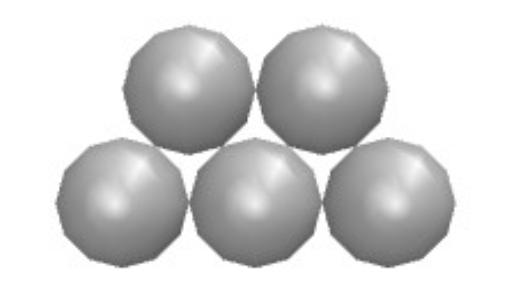
\includegraphics[width=0.25\linewidth]{Figures/fen5}
\caption{Geometry for $m_{s}=5$}
\label{fig:fen5}
\end{figure}

The minimization was done using the Particle Swarm Optimization (PSO) method with the following objective function:
\begin{equation}
\min\limits_{\sigma,\epsilon,\lambda_{r}} F_{obj}(\sigma,\epsilon,\lambda_{r})= \sum_{i=1}^{N_{p}} \left(\frac{P_{v}^{SAFT}(T_{i},\sigma,\epsilon,\lambda_{r})-P_{v}^{exp}(T_{i})}{P_{v}^{exp}(T_{i})} \right)^2
\label{eqn:fobjm}
\end{equation}

The $P_{v}^{exp}$ is the experimental vapor pressure and $P_{v}^{SAFT}$ is the vapor pressure obtained with SAFT-VR Mie EoS. The method used to calculate the bubble point with the EoS was the one proposed by \citeonline{smithbook}. The resulting  parameters $\sigma$, $\epsilon $ and $\lambda _{r}$ from this minimization are the final force field parameters used in molecular simulations. The parameterization with the \citeonline{lafitte2012} ring equation was done with $m_{s}=3$ so every bead would represent one ring:

\begin{figure}[th]
	\centering
	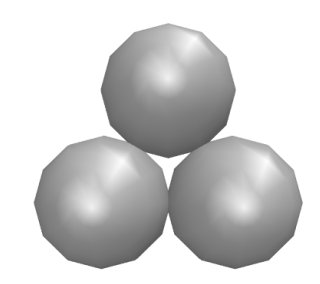
\includegraphics[width=0.15\linewidth]{Figures/fe3}
	\caption{Geometry for $m_{s}=3$}
	\label{fig:fen3}
\end{figure}

The first part of the estimation followed the same procedure described above for the \citeonline{muller2017} equation. As explained in section \ref{parsaft}, the \citeonline{lafitte2012} equation requires the estimation of the correction factors $c_{\sigma}$ and $c_{\epsilon}$ (Eqs. \eqref{eqn:csigma} and \eqref{eqn:ceps}). The PSO method was also used and the objective function is the one in Eq. \eqref{eqn:fobjla}. In this equation, the vapor pressures and saturated liquid densities from molecular simulations were obtained using the Gibbs Ensemble Monte Carlo method on the NVT ensemble  (section \ref{gemc}).

The boxes for the simulations on the GEMC-NVT were generated inserting 400 molecules on the liquid box and 100 on the vapor one using the Packmol package \cite{packmol}. The initial densities of each box were given the value of the saturated densities found with the SAFT-VR Mie Eos to avoid the migration of all molecules to a single phase throughout the simulation. The equilibration and production time consisted of $10^{4}$ and $5 10^{4}$ MC cycles respectively. Each MC cycle corresponded to $10^3$ rotation trials, $10^3$ translation trials, $10^2$ molecule insertion trials, $10^2$ molecule deletion trials and 10 volume exchange trials. The cut off distance was equal to $20 \hat{A}$ with no long range interactions. The saturated vapor density ($\rho_{vap}$), the saturated liquid density ($\rho_{liq}$) and the vapor pressure ($P_{v}$) were sampled at each 100 MC cycles and this data were divided in five blocks to calculate the averages and standard deviations. The corrections found after the estimations was then used to calculate the of $\sigma$ and $\epsilon$ parameters to use in molecular simulations with Eqs. \eqref{eqn:simsigma} and \eqref{eqn:simeps}.

\section{Solvation Free energy Calculations}\label{solvme}

The molecular dynamic simulations to estimate the free energy differences with the SAFT-$\gamma$ Mie force field were performed using the Lammps package \cite{lammps}. The motion equations were integrated with the velocity-Verlet algorithm \cite{verlet} with a time step of 1 fs. The molecules were treated as rigid bodies, as required by the coarse grained model. The thermostat and the barostat were the Nose/Hoover with chains with a damping factors of 100 and 1000 fs respectively. The SAFT-$\gamma$ Mie model doesn't consider electrostatics interactions explicitly, hence there was no shifting of forces or long range corrections. The potential cutoff was equal to 20 $\dot{A}$ \cite{muller2017} with a neighbor skin of 2 $\dot{A}$. The initial configuration of the  solvated systems were generated with the Packmol package \cite{packmol}. For the binary mixtures, one molecule of solute and a varying number of solvent molecules- 700 molecules for toluene and octanol, 1024 for hexane, 3000 for water - were randomly added to a cubic box. The simulations to study solvation free energy of phenanthrene in a mixture of toluene and carbon dioxide were done with different fractions of carbon dioxide. The  system consisted of one molecule of phenanthrene for all the fractions and 123 molecules of $CO_{2}$ and 618 molecules of toluene for $w_{CO_{2}} = 0.087$; 166 molecules of $CO_{2}$; 589 molecules of toluene for $w_{CO_{2}} = 0.119$; 232 molecules of $CO_{2}$ and 545 molecules of toluene for $w_{CO_{2}} = 0.169$ and 380 molecules of $CO_{2}$ and 446 molecules of toluene for $w_{CO_{2}} = 0.289$.

All simulations were carried out maintaining the temperature and pressure constant at 298 K and 1 bar, except the ones containing carbon dioxide. These were performed at 298 K and at the pressure of the liquid phase equilibrium correspondent to the $CO_{2}$ fraction \cite{co2toliq}. For all the simulations, the initial box was equilibrated at the NPT ensemble for 2 ns and then the resulting configurations were used on the alchemical simulations. These were carried out with the Lammps user package for alchemical simulations with the Mie Potential developed by our group, available at https://github.com/atoms-ufrj/USER-ALCHEMICAL. In the simulations, the sampling of a new state was tried at every 10 MD steps. In order to define the optimal values of $\lambda$ and $\eta$ related to each state, short trials simulations, lasting around 10 ns, were carried out. In the first simulation, the group of $\lambda$ for all the pairs solvent-solute was: (0.0,0.15,0.2,0.25,0.3,0.4,0.45,0.5,0.55,0.7,0.9,1.0) and the $\eta s$ were set to zero or were given the values of the ones found for similar mixtures. The subsequent groups of $\eta$ were estimated  with the flat histogram approach (Eq. \eqref{eqn:weight}) using the solvation free energy values stemming from the previous simulations. The results with the new weights were then utilized to optimize the group of $\lambda s$ by minimizing the number of round trips as described in section \ref{ee}. The $\eta s$ correspondent to the newest group of $\lambda s$ were interpolated from free energy differences. With the final values of $\eta$ and $\lambda $ defined for each mixture, larger simulations with a time of 20 ns were performed. 

Since the force field considers that the beads don't have charges, there is no coulombic interaction and Eq. \eqref{eq:freesolv} becomes equal to $\Delta G_{3 \rightarrow 4} $. The post processing method used to calculate free energy differences was the Multisate Bennet Acceptance Ratio (MBAR) described in section \ref{mbar}. The software alchemical-analysis \cite{klimovich} was used to obtain the $\Delta G_{solv}$ with MBAR and to assess the results quality. The binary interaction  parameter of Eq. \eqref{eqn:epsmix} was only estimated for pairs with water as a solvent. The strategy picked was to carry out the simulations described above in three values of $k_{ij}$ and then refine the parameter until a value in good agreement with the experimental solvation free energy was found. The estimation was not carried out with the SAFT VR Mie EOS because the $k_{ij}$ obtained  with this strategy gave poor results for the free energy.


%72 molecules of $CO_{2}$ and 652 molecules of toluene for $x_{CO_{2}} = 0.1$;


